\documentclass[12pt, a4paper, oneside]{book} 
\usepackage{svn-multi}
\usepackage{makecell}

\tolerance=10000
\vfuzz=8pt

\usepackage{lipsum}

\usepackage{silence}
\WarningFilter{hyperref}{Invalid value `0'}
\WarningFilter{latex}{Some font shapes were not available, defaults substituted.}
\usepackage{amsmath}

\svnid{$Id$}
\usepackage{prelim2e}
\renewcommand{\PrelimWords}{Draft Copy \svnkw{Id}}

%%\newcommand*{\mysvnrev}{\svnrev}
\usepackage[hyperindex=true,
			bookmarks=true,
            pdftitle={}, pdfauthor={Olivia Walters},
            colorlinks=false,
            pdfborder=0,
            pagebackref=false,
            citecolor=blue,
            plainpages=false,
            pdfpagelabels,
            pagebackref=true,
            hyperfootnotes=false]{hyperref}
\usepackage[all]{hypcap}
\usepackage[palatino]{anuthesis}
\usepackage{afterpage}
\usepackage{graphicx}
\usepackage{thesis}
\usepackage[square]{natbib}
\usepackage[normalem]{ulem}
\usepackage[table]{xcolor}
\usepackage{makeidx}
\usepackage{cleveref}
\usepackage[centerlast]{caption2}
\usepackage{float}
\urlstyle{sf}
\renewcommand{\sfdefault}{cmr}
\usepackage[T1]{fontenc}
\usepackage[scaled]{beramono}

\usepackage{multirow}


\renewcommand*{\backref}[1]{}
\renewcommand*{\backrefalt}[4]{
  \ifcase #1 %
    %
  \or
    (cited on page #2)%
  \else
    (cited on pages #2)%
  \fi
}




%      $Id: macros.tex 506 2009-10-05 16:57:07Z daniel $    

\usepackage{booktabs}
\usepackage{relsize}
\usepackage{xspace}
\usepackage{subfigure}
\usepackage{listings}
\lstloadlanguages{java}
\DeclareGraphicsRule{*}{pdf}{*}{}
\newcommand{\otoprule}{\midrule[\heavyrulewidth]}
\newcommand{\pldi}{ACM Programming Language Design and Implementation (PLDI)}
\newcommand{\taco}{ACM Transactions on Architecture and Code Optimization (TACO)}
\newcommand{\lctes}{ACM Languages, Compiler, and Tool Support for Embedded Systems (LCTES)}
\newcommand{\popl}{ACM Principles of Programming Languages (POPL)}
\newcommand{\ecoop}{European Conference for Object-Oriented Programming (ECOOP)}
\newcommand{\asplos}{ACM Architectural Support for Programming Languages and Operating Systems (ASPLOS)}
\newcommand{\sigmetrics}{ACM Measurement and Modeling of Computer Systems (SIGMETRICS)}
\newcommand{\oopsla}{ACM Object-Oriented Programming, Systems, Languages, and Applications (OOPSLA)}
\newcommand{\ismm}{International Symposium on Memory Management (ISMM)}
\newcommand{\veee}{ACM/USENIX Virtual Execution Environments (VEE)}
\newcommand{\micro}{ACM/IEEE International Symposium on Microarchitecture}
\newcommand{\isca}{ACM/IEEE International Symposium on Computer Architecture (ISCA)}
\newcommand{\icse}{International Conference  on Software Engineering (ICSE)}
\newcommand{\pact}{Parallel Architectures and Compilation Techniques (PACT)}
\newcommand{\casess}{ACM Compilers, Architectures, and Synthesis for Embedded Systems (CASES)}

\definecolor{tableheadcolor}{rgb}{0.8,0.8,1.0}
%\definecolor{tablealtcolor}{rgb}{0.9,0.9,1.0}
\definecolor{tablealtcolor}{rgb}{0.9,0.9,0.95}


\definecolor{todocolor}{rgb}{0.8,0.8,1.0}
\definecolor{fixcolor}{rgb}{1,0.8,0.8}
\definecolor{commentcolor}{rgb}{0.8,1.0,0.8}


\newcommand{\listingfigure}[3]{
\begin{figure}[ht!]
  \begin{center}
    \begin{minipage}[t]{\textwidth-4cm}
      \lstinputlisting{#1}
    \end{minipage}
  \end{center}
  \caption{#3}#2
\end{figure}}

\newcommand{\includeabchart}[5]{
\begin{figure}[ht!]
\begin{center}
\newcommand{\atitle}{#4}
\newcommand{\btitle}{#5}
\input{charts/#1.tex}
\end{center}
\caption{#3}#2
\end{figure}}

\newcommand{\placeholderfigure}[2]{
\begin{figure}[ht!]
  \begin{center}
    \resizebox{\textwidth-2cm}{0.7\textwidth-1.4cm}{todo}
  \end{center}
  \caption{#2}#1
\end{figure}}

\newcommand{\singlegraphfigure}[3]{
\begin{figure}[ht!]
  \begin{center}
    \includegraphics[width=\textwidth-2cm]{#1}
  \end{center}
  \caption{#3}#2
\end{figure}}

\usepackage[color=todocolor, colorinlistoftodos]{todonotes}

%\newcommand{\notinpart}{%
% \def\toclevel@chapter{-1}\def\toclevel@section{0}\def\toclevel@subsection{1}} \newcommand{\inpart}{
% \def\toclevel@chapter{0}\def\toclevel@section{1}\def\toclevel@subsection{2}}


%
% Stuff for pretty printing the source code using listings.sty
%


%% set Java as the default language
\lstset{
  numbers=left,
  numberstyle=\tiny,
  stepnumber=1,
  numbersep=2em,
  language=java,                         % the language
  basicstyle=\footnotesize\ttfamily,     % the basic font family to use
  commentstyle=\itshape,                 % the font for comments
  stringstyle=\ttfamily,
%  morekeywords={@Intrinsic, @Unboxed, @RawStorage}
}
%\lstset{language=java}

\newcommand{\textjava}[1]{{\lstset{basicstyle=\ttfamily}\lstinline@#1@}}
\newcommand{\textjavafn}[1]{{\lstset{basicstyle=\footnotesize\ttfamily}\lstinline@#1@}}
%\usepackage{lstasm}
\usepackage{setspace}
\usepackage{ifthen}
%\usepackage{color}
%\usepackage{smallheadings}

\long\def\sfootnote[#1]#2{\begingroup%
\def\thefootnote{\fnsymbol{footnote}}\footnote[#1]{#2}\endgroup}
%
% code
%

\newcommand{\address}{\textjava{Address}\xspace}
\newcommand{\ubregion}{\textjava{unbump-region()}\xspace}
\newcommand{\word}{\textjava{Word}\xspace}
\newcommand{\freeme}{\textjava{free()}\xspace}
\newcommand{\freemeunbump}{\textjava{unbump()}\xspace}
\newcommand{\freemeunbumpregion}{\textjava{unbump-region()}\xspace}
\newcommand{\freemeunreserve}{\textjava{unreserve()}\xspace}

%
% abbreviations
%


\newcommand{\eg}{e.g., }
\newcommand{\ie}{i.e., }

\newcommand{\GenMS}{\emph{GenMS}\xspace}
\newcommand{\GenImmix}{\emph{GenIX}\xspace}
\newcommand{\mmtk}{MMTk\xspace}
\newcommand{\jikes}{Jikes RVM\xspace} 
\newcommand{\jikesrvm}{\jikes} 
\newcommand{\jala}{Jalape\~{n}o\xspace} 
\newcommand{\jalapeno}{Jalape\~{n}o\xspace} 

\newcommand{\dacapo}{\textsf{DaCapo}\xspace}
\newcommand{\specjvm}{\textsf{SPECjvm98}\xspace}
\newcommand{\cattrack}{\textsf{cattrack}\xspace}
\newcommand{\spec}{\textsf{SPEC}\xspace}

\newcommand{\nurserytype}[1]{{\fontfamily{cmss}\selectfont \textsl{#1}}}
\newcommand{\alloc}{\nurserytype{allocate}\xspace}
\newcommand{\collect}{\nurserytype{collect}\xspace}
\newcommand{\redirect}{\nurserytype{redirect}\xspace}

\newcommand{\bmtype}[1]{{\textsf{#1}}}

\newcommand{\jbb}{\bmtype{jbb2000}\xspace}
\newcommand{\psjbb}{\bmtype{pjbb2005}\xspace}
\newcommand{\pjbb}{\bmtype{pjbb2005}\xspace}
\newcommand{\specjbb}{\bmtype{SPECjbb2005}\xspace}
\newcommand{\jess}{\bmtype{jess}\xspace}
\newcommand{\raytrace}{\bmtype{raytrace}\xspace}
\newcommand{\db}{\bmtype{db}\xspace}
\newcommand{\javac}{\bmtype{javac}\xspace}
\newcommand{\jack}{\bmtype{jack}\xspace}
\newcommand{\compress}{\bmtype{compress}\xspace}
\newcommand{\mpegaudio}{\bmtype{mpegaudio}\xspace}
\newcommand{\mtrt}{\bmtype{mtrt}\xspace}
\newcommand{\antlr}{\bmtype{antlr}\xspace}
\newcommand{\bloat}{\bmtype{bloat}\xspace}
\newcommand{\chart}{\bmtype{chart}\xspace}
\newcommand{\eclipse}{\bmtype{eclipse}\xspace}
\newcommand{\fop}{\bmtype{fop}\xspace}
\newcommand{\hsqldb}{\bmtype{hsqldb}\xspace}
\newcommand{\jython}{\bmtype{jython}\xspace}
\newcommand{\luindex}{\bmtype{luindex}\xspace}
\newcommand{\lusearch}{\bmtype{lusearch}\xspace}
\newcommand{\Lusearch}{\bmtype{Lusearch}\xspace}
\newcommand{\pmd}{\bmtype{pmd}\xspace}
\newcommand{\ps}{\bmtype{ps}\xspace}
\newcommand{\SPECjbb}{\bmtype{SPECjbb}\xspace}
\newcommand{\xalan}{\bmtype{xalan}\xspace}
\newcommand{\sunflow}{\bmtype{sunflow}\xspace}
\newcommand{\Sunflow}{\bmtype{Sunflow}\xspace}
\newcommand{\avrora}{\bmtype{avrora}\xspace}
\newcommand{\core}{Core2 Quad\xspace}
\newcommand{\corelong}{Intel Core2 Quad Q6600\xspace}
\newcommand{\phenom}{Phenom II\xspace}
\newcommand{\phenomlong}{AMD Phenom II X6 1055T\xspace}
\newcommand{\sandy}{i7-2600\xspace}
\newcommand{\sandylong}{Intel Core i7-2600\xspace}



\newcommand{\ghostscript}{\bmtype{ghostscript}\xspace}

\newcommand{\doi}[1]{\href{http://dx.doi.org/#1}{\nolinkurl{doi:#1}}}
%
% misc
%
\newcommand{\fix}[1]{\todo[color=fixcolor]{#1}}
\newcommand{\comment}[1]{\todo[color=commentcolor]{#1}}
\newcommand{\ifix}[1]{\todo[inline,color=fixcolor]{#1}}
\newcommand{\icomment}[1]{\todo[inline,color=commentcolor]{#1}}
\newcommand{\itodo}[1]{\todo[inline]{#1}}
\newcommand{\ignore}[1]{}
\newcommand{\mccenter}[1]{\multicolumn{1}{c|}{#1}}

%
% figure spacing
%
%\clubpenalty 10000
%\widowpenalty 10000
%\def\topfraction{0.9}
%\def\bottomfraction{0.9}
%\def\textfraction{0.1}
%\renewcommand{\singlespacing}{\renewcommand{\baselinestretch}{1.00}\small\normalsize}
%\renewcommand{\doublespacing}{\renewcommand{\baselinestretch}{1.5}\small\normalsize}
%\newcommand{\tight}{\renewcommand{\baselinestretch}{1.28}\small\normalsize}
%\renewcommand{\subfigbottomskip}{0.25ex}
%\renewcommand{\subfigcapskip}{0ex}
%\renewcommand{\subfigcapskip}{-1ex}
%\newcommand{\subfigshrink}{-0.75ex}
%\newcommand{\subfigcapspace}{2ex}

%\newcommand{\subwidth}[0]{.32\textwidth}


%
% margins
%
%\topmargin -.5truein
%\textheight 9truein
%\oddsidemargin .25truein
%\evensidemargin .25truein
%\textwidth 6truein


%
% crossreferencing footnotes
%
%\newcommand{\fnref}[1]{~(\ref{#1})}
%\newcommand{\onecolparbox}{3.1in}


%\newcommand{\textjava}[1]{{\lstset{language=java,basicstyle=\footnotesize\ttfamily}\lstinline@#1@}}
%\newcommand{\textasm}[1]{{\lstset{language=asm,basicstyle=\footnotesize\ttfamily}\lstinline@#1@}}

%%
%% Change the sections etc.
%%
%\makeatletter
%\parskip=0pt
%\renewcommand\section{\@startsection{section}{1}{\z@}%
%                                   {-2.5ex}% beforeskip
%%                                   {1ex}% afterskip
%                                   {\large \bfseries \raggedright}}
% \renewcommand\subsection{\@startsection{subsection}{2}{\z@}%
%                                     {-2ex\@plus -1ex \@minus -.2ex}%
%                                      {.5ex \@plus .2ex}%
%                                      {\normalsize \bfseries \raggedright}}
% \renewcommand\subsubsection{\@startsection{subsubsection}{3}{\z@}%
%                                      {-2ex\@plus -1ex \@minus -.2ex}%
%                                      {1ex \@plus .2ex}%
%                                      {\normalfont\fontsize{11pt}{12pt}\selectfont\itshape}}
%\renewcommand{\thesubsubsection}{\thesubsection.\arabic{subsubsection}}

%\renewcommand\paragraph{\@startsection{paragraph}{4}{\z@}% 
%  {.5em}%
%  {-1em}%
%  {\normalfont\normalsize\bfseries\parskip=0pt}}
%\setlength\partopsep{0\p@}
%\setlength\parskip{0\p@ \@plus \p@}

%\makeatother
%\parindent=9pt





%%% Local Variables: 
%%% mode: latex
%%% TeX-master: "doa"
%%% End:
            
%%%%%%%%%%%%%%%%%%%%%%%%%%%%%%%%%%%%%%%%%%%%%%%%%%%%%%%%%%%%%%%%%%%%%%%
%% Preamble
\title{Magnetic fields in circumgalactic HVCs}
\author{Olivia Walters}
\date{\today}

\renewcommand{\thepage}{\roman{page}}

\makeindex
\begin{document}

\hbadness=10000

%\doparttoc
%%%%%%%%%%%%%%%%%%%%%%%%%%%%%%%%%%%%%%%%%%%%%%%%%%%%%%%%%%%%%%%%%%%%%%%
%% Title page
\pagestyle{empty}
\thispagestyle{empty}
%% anuthesis.sty Copyright (C) 1996, 1997 Steve Blackburn
%% Department of Computer Science, Australian National University
%%

\begin{titlepage}
  \enlargethispage{2cm}
  \begin{center}
    \makeatletter
    \Huge\textbf{\@title} \\[.4cm]
    \Huge\textbf{\thesisqualifier} \\[2.5cm]
    \huge\textbf{\@author} \\[9cm]
    \makeatother
%%   \LARGE A thesis submitted for the degree of \\
%%    Master of Philosophy at \\
%%    The Australian National University \\[2cm]
    \LARGE A thesis submitted for the degree of \\
    Test Github integration \\
    The Australian National University \\[2cm]
    \thismonth
  \end{center}
\end{titlepage}


%%%%%%%%%%%%%%%%%%%%%%%%%%%%%%%%%%%%%%%%%%%%%%%%%%%%%%%%%%%%%%%%%%%%%%%
%% Here begin the preliminaries
\vspace*{14cm}
\begin{center}
  \makeatletter
  \copyright\ \@author{} 2024
  \makeatother
\end{center}
\noindent
\begin{center}
  \footnotesize{~} %\aboutthesis
\end{center}
\noindent

\newpage

\addcontentsline{toc}{chapter}{Statement of Originality}

\vspace*{7cm}
\begin{center}
  Except where otherwise indicated, this thesis is my own original
  work.
\end{center}

\vspace*{4cm}

\hspace{8cm}\makeatletter\@author\makeatother\par
\hspace{8cm}\today


%%%%%%%%%%%%%%%%%%%%%%%%%%%%%%%%%%%%%%%%%%%%%%%%%%%%%%%%%%%%%%%%%%%%%%%
%% Dedication
%\cleardoublepage
%\pagestyle{empty}
%\vspace*{7cm}
\begin{center}
  To my grandmother, Hilda Filipovic, for being a very important person in my life, and a rock on which I relied on in the process of completeing my honours year.
\end{center}

\vspace*{4cm}

%%%%%%%%%%%%%%%%%%%%%%%%%%%%%%%%%%%%%%%%%%%%%%%%%%%%%%%%%%%%%%%%%%%%%%%
%% Acknowledgements
\cleardoublepage
\pagestyle{empty}
\chapter*{Acknowledgments}
\addcontentsline{toc}{chapter}{Acknowledgments}


I would like to thank my primary and secondary supervisors, Dr. Craig Anderson and Prof. Naomi-McClure Griffiths for being the main body of support, data, and ideas when writing this thesis. I would also like to acknowledge Prof. Brian Gaensler and Dr. Lyla Jung for providing further aid in the process of analysis, and their support in regards to POSSUM itself. The ASKAP POSSUM team more broadly has come as a great aid and source of community during the production of this thesis.

Fellow radio astronomer Callum Lynn has also been a great source of advice and help in constructing this thesis for a more general astronomical audience, along with his guidance about the honours and PhD process.

The ANU SSN Consultancy Group was a crucial part in the validation of the statistical techniques listed in this paper, including the suggestion to use the Weighted ANOVA and Tukey HSD test.

I would also like to thank my grandmother, Hilda Filipovic, for being a very important person in my life, and a rock on which I relied on in the process of completeing my honours year.

%%%%%%%%%%%%%%%%%%%%%%%%%%%%%%%%%%%%%%%%%%%%%%%%%%%%%%%%%%%%%%%%%%%%%%%
%% Abstract
\cleardoublepage
\pagestyle{headings}
\chapter*{Abstract}
\addcontentsline{toc}{chapter}{Abstract}
\vspace{-1em}

\lipsum[1]

%%% Local Variables: 
%%% mode: latex
%%% TeX-master: "paper"
%%% End: 

%%%%%%%%%%%%%%%%%%%%%%%%%%%%%%%%%%%%%%%%%%%%%%%%%%%%%%%%%%%%%%%%%%%%%%%
%% Table of contents
\cleardoublepage
\pagestyle{headings}
\markboth{Contents}{Contents}
\tableofcontents
\listoffigures
\listoftables

%%%%%%%%%%%%%%%%%%%%%%%%%%%%%%%%%%%%%%%%%%%%%%%%%%%%%%%%%%%%%%%%%%%%%%
%% Here begins the main text
\mainmatter

%% Introduction
\chapter{Introduction}
\label{cha:introduction}

The question of how gas is accreted into galaxies fuelling star-formation is a puzzle that has perplexed astronomers for decades \citep{ID28,ID23}. Due to the complexities in the structures of star-forming galaxies, there are many factors involved in the process of, and potential sources of accretion. What astronomers do know, at least, is that star-forming galaxies require a continuous supply of fresh gas to continue their star formation \citep{ID28,ID23, ID19}.


Due to observational constraints, astronomers are required to attempt to answer this question by examining the behaviours of our own Milky Way and Local Group environment, assuming the Milky Way is typical of a star-forming galaxy.


A major factor to consider when answering this question is where fresh pristine gas comes from, and by what mechanism it takes to enter the disks of star-forming galaxies \citep{ID8, ID28, ID49}. High Velocity Clouds (HVCs) have been a suggested mechanism for Galactic gas accretion and this report aims to evaluate the viability of this suggestion \citep{ID3,ID19}. 


\section{High Velocity Clouds}
\label{sec:hvcs}

HVCs are clouds of gas found in the Milky Way's Circumgalactic Medium (CGM) and Galactic halo. They have a high peculiar velocity relative to the Galactic Standard of Rest (GSR), typically 70-90 $\mathrm{km s^{-1}}$ \citep{ID7, ID8}. As will be shown in section \ref{ssec:draping}, this increased speed, and its interaction with halo magnetic fields, is hypothesized to allow the HVC to survive as it travels through the CGM and halo so it can reach the Galactic disk and Interstellar Medium (ISM) of the Milky Way.


There are a few hypothesises as to where HVCs originate. \cite{ID19} suggests that HVCs originate from the Intergalactic Medium (IGM) surrounding the local group. However, there is also a belief that some HVCs likely 'tore off' from satellites like the Magellanic Clouds, due to the presence of their own dark matter subhaloes, and the existence of HVCs in the Magellanic Stream and Leading Arm \citep{ID27, ID2}. Recent simulations from TNG50 have indicated that HVCs mainly have their origins in the warm-hot CGM, formed through cooling from thermal instabilities \citep{ID74}.


HVCs typically have a neutral mass gas content of $10^5 - 3\times10^5 M_{\odot}$ \citep{ID19}. They are generally shaped like comets, with a primary bulb that is approximately 0.5-25 kpc in diameter - a value that is highly dependent on distance to the Galactic midplane, which can range from approx. 2 kpc - 15 Mpc \citep{ID19, ID13}. Furthermore, HVCs have tail-like structures that account for one eighth the baryonic mass of the HVC \citep{ID13}. These tails leave behind long streams of gas that remain after collision with the Galactic disk \citep{ID19}. This size-distance correlation, comet-like structure, and long streaming tails suggest quite conclusively that HVCs shed large quantities of material as they make their journey to the ISM.


Figure \ref{fig:hvc_example} is from \cite{ID13}, which provides a typical example of what a HVC looks like in HI, specifically using the example of HVC125+41-207.

\begin{figure}
    \includegraphics[width=12cm]{"Konz_2002.png"}
    \centering
    \caption{From \cite{ID13}, figure 2. An example of a typical HVC shape and structure, specifically that of HVC125+41-207. The contour lines and shading indicate HI column density.}
    \label{fig:hvc_example}
\end{figure}


\section{Magnetic Fields}
\label{sec:bfields}

The primary issue facing HVCs as an explanation for gas accretion is its capacity to survive as it travels through the CGM and Galactic halo. As discussed, in section \ref{sec:hvcs}, HVCs can loose a lot of size and mass as it approaches towards the Galactic disk, with the long trails it leaves behind being evidence for ram-pressure stripping as the HVC collides with the gas present in the halo \citep{ID11, ID23, ID33}. \cite{ID25} demonstrates that without anything to counter this effect, HVCs with masses under $10^{4.5} M_{\odot}$ would completely disperse within 10 kpc of halo travel.


Additionally, HVCs are subject to Kelvin-Helmholtz (K-H) instabilities, which is triggered by the nature of the HVC being a cloud of warm gas travelling at high speeds through a medium of warm halo gas. These K-H instabilities are a significant factor that would lead a to HVC dispersing before it reaches the Galactic disk \citep{ID11, ID23, ID33}.


\subsection{Draping}
\label{ssec:draping}

The proposed solution to handle this problem is magnetic fields. The Galactic halo is magnetised to some degree \citep{ID30, ID16, ID4, ID42}. It is hypothesised that HVCs accumulate these existing magnetic fields in the Galactic halo, causing them to cloak the HVC with a shield that protects against ram pressure stripping and supresses K-H instabilities \citep{ID10, ID11, ID13, ID23, ID24, ID34}. This phenomenon is referred to as 'magnetic draping'.


There is not enough observational evidence to support the magnetic draping hypothesis. However, with recent advancements in: RM radio surveys \citep{ID52, ID71, ID1, ID3, ID6, ID18, ID43, ID44, ID45}; the analysis of ram pressure stripping \citep{ID11, ID23, ID33}; measurement and estimation of magnetic fields \citep{ID5, ID23, ID30, ID11, ID26, ID21}; and simulations of HVCs \citep{ID13, ID23, ID24, ID33, ID34} – it is now possible to attempt to observe and analyse the role of magnetic draping in HVCs observationally.


Previous and recent simulations involve reports produced by \cite{ID23, ID24, ID33} (henceforth referred to as the “\citeauthor{ID23} simulations”) that provide detailed insight onto how a magnetic draping protects HVCs from collapse, complementing earlier work by \cite{ID13, ID11}. It is shown from the \citeauthor{ID23} simulations that magnetic fields of about 0.3-1 {\textmu}G can provide stability to HVCs.


However, increasing magnetic field strength beyond a certain threshold can result in less stability; magnetic fields can accelerate the effects of Rayleigh-Taylor (R-T) instabilities and the magnetic pressure applied by the draped fields can also slow down a HVC to the point that it no longer is fast enough to sweep up these magnetic fields. From the \citeauthor{ID23} simulations, the upper threshold where these effects start increasing instability is about 1 {\textmu}G (specifically stating a maximum of approx. 3 {\textmu}G), thus HVCs should ideally have a “Goldilocks” magnetic field strength on the order of magnitude of 0.1{\textmu}G, with 1{\textmu}G being too high, and 0.01{\textmu}G being too low.


The effectiveness of magnetic draping is affected by the morphology of these fields and the physical properties of the HVC. The \citeauthor{ID23} simulations state that both the orientation of the magnetic field with respect to the direction of motion of the HVC, and where the magnetic field is located are important considerations. It is expected that HVC is not entirely covered in a magnetic field, only the part that is front facing in the direction of travel. While it is possible to draw conclusions about the survivability of a HVC from the strength of the magnetic field, modelling is required to confirm the accuracy of such conclusions \citep{ID5}. The \citeauthor{ID23} simulations also predict that metallicity can affect the HVC's survivability, via affecting phase transitions, with high-density metal-rich clouds and low-density metal-poor clouds being more unstable than HVCs of the opposite compositions.


The simulations by \cite{ID36} predict higher magnetic field strengths on the order of 1 \textmu G. It is very clear that even simulationaly, the specific strengths of magnetic fields surrounding HVCs have high uncertainty. The results of this report will still compare against the \citeauthor{ID23} simulations despite this.


\subsection{Faraday Rotation}
\label{ssec:faraday}

Magnetic fields cannot directly be imaged by a telescope. Instead, researchers can use the phenomenon of Faraday Rotation to quantify the line-of-sight magnetic field strength. Polarised radiation tends to rotate as it travels through a medium with a magnetic field present. This effect is quantified by equation \ref{eq:stokes}.

\begin{equation}
    \Delta\psi = \phi\lambda^2
    \label{eq:stokes}
\end{equation}


Where $\lambda$ is the wavelength of radiation, $\phi$ is the faraday depth and $\Delta\psi$ is the change in polarisation angle. Thus, by recording the stokes parameters of incoming light from distant radio sources, one can derive the Rotation Measure (RM) of incoming radiation, which is a statistical quantifier of Faraday Rotation and faraday depth \citep{ID1, ID14}. For the purposes of this report, rotation measure and faraday depth are treated as equivalent henceforth, despite their subtle differences.


For illustrative purposes, a schematic diagram of how Faraday Rotation is measured by telescopes on Earth with the aim of analysing HVCs are shown in figure \ref{fig:schema}.


\cite{ID1} describes the method by which this report's main source, the Polarisation Sky Survey of the Universe's Magnetism (POSSUM), obtained its RMs from radio observations. There is a direct connection between RM and line-of-sight magnetic field strength, quantified by equation \ref{eq:rm_integral} \citep{ID5, ID1, ID26, ID27, ID30}.


\begin{equation}
    \mathrm{RM} = 0.812 \int_{s_{\mathrm{observer}}}^{s_{\mathrm{source}}}{\frac{n_e(s)}{\mathrm{cm^{-2}}}\frac{B_{\parallel}}{\mu\mathrm{G}}\frac{ds}{\mathrm{pc}}} \mathrm{rad~m^{-2}}
    \label{eq:rm_integral}
\end{equation}


In which, $B_{\parallel}$ is the magnetic field strength, $\mathrm{RM}$ is the Rotation Measure, and $n_e$ is the electron density of the medium as a function of line-of-sight distance $s$. The analysis of this equation, its solutions, and the use of it in calculating the magnitude of line-of-sight magnetic fields is discussed in section \ref{cha:derivation}.


Faraday Rotation also occurs in the ISM of the Milky Way, due to the slight magnetisation of the ISM \citep{ID37, ID30, ID21}. This magnetisation is antisymmetric with galactic longnitude \citep{ID30}. Hence it is also important to remove the foreground from RM observations.


When making radio observations of RMs, a principal factor to consider is the observational signal to noise ratio and detector sensitivity. Radio sources tend to appear in the field after high exposure times as point-like sources. These point-like sources are then collated into an “RM grid” which has a particular density measured in sample points per square degree. The sensitivity of a detector and total integration time determines the number of source points observed as seen in figure \ref{fig:loi} \citep{ID59}.

\begin{figure}
    \includegraphics[width=9cm]{"Loi_2019.png"}
    \centering
    \caption{From \cite{ID59}, figure 4. A graph of the relationship between the sensitivity at 1.4 GHz (x-axis) and the average mimumum number of RM sample points per square degree (y-axis). The black points are not relevant to the report, but the purple line and equation describe the determined relationship.}
    \label{fig:loi}
\end{figure}

Signal to noise is of primary concern when measuring the effect of Faraday Rotation. At low enough signal-to-noise ratios, it is possible to encounter noise peaks which do not accurately represent the real RM \citep{ID60}. Figure \ref{fig:snr} gives a visual illustration of this phenomenon. The issue in question is that any observation of RM grids is going to dip below the signal-to-noise threshold of approx. 6, which can introduce an intrinsic scatter in collected RM grid data. Thus RM points below this threshold are ignored. However, the dataset masks out all RMs below a signal to noise of 8, which is considered conservative \citep{ID71}.

As will be discussed in section \ref{sec:ASKAP}, the POSSUM dataset is the first dataset with 30 RMs per square degree versus legacy surveys which had only 1 RM per square degree.

\begin{figure}
    \includegraphics[width=12cm]{"Macquart_2012.jpg"}
    \centering
    \caption{From \cite{ID60}, figure 1. A graph displaying the effect of observational (stokes parameters) signal-to-noise ratio the resultant faraday depth on a sample set of observations.}
    \label{fig:snr}
\end{figure}

\begin{figure}
    \includegraphics[width=10cm]{"Schematic Diagram.png"}
    \centering
    \caption{An schematic diagram illustrating how the RM of incoming radio radiation is observed, notably around HVCs. Note that the extragalactic radiation will appear as randomly distributed across the field of view.}
    \label{fig:schema}
\end{figure}

\subsection{Temperature, Chemical Properites, and Emission}
\label{sec:chem}

Due to their hypothesised origins in extragalactic gas, HVCs contain mostly hydrogen gas such as HI, which can be seen with 21 cm emission \citep{ID7, ID8, ID6}. The proportion of ionised gas in HVCs is still heavily debated. HVCs also emit H-alpha, however due to extinction effects, it is difficult to observe \citep{ID9, ID43}.

HVCs have a temperature relationship with proximity to the Galactic midplane, with an average HVC temperature of 10000 K and a range of temperatures ranging from 8000 – 12000 K \citep{ID49, ID48}. The temperature of a HVC is in the region in which atomic hydrogen transitions from neutral (HI) to ionised (HII), suggesting that HVCs may be partly ionised \citep{ID49, ID48, ID68}. This temperature relationship is dependent on their position with respect to the Galactic midplane, with HVCs closer to the midplane generally being cooler \citep{ID48}. This temperature is contrasted by the Galactic halo temperature, which varies from $\approx 10^4-10^6$ K \citep{ID19}. This is an important factor in creating K-H instabilities.


There is evidence that HVCs can contain alpha group elements. \cite{ID49, ID48} found the presence of [NII] 6583{\AA}, [SII] 6716{\AA}, and [OIII] 5007{\AA} emission lines – with a conclusion that Nitrogen abundance is 0.15-0.44 times solar abundance levels. The observation of these emission lines can help constrain the metallicity of any HVC  \citep{ID49}. Metallicity is important in both how HVCs act as fresh gas supplies for star formation. As well as the mechanism by which HVCs can survive their transit through the CGM \citep{ID24}; more on the latter in section \ref{ssec:draping}. While HVCs can contain heavier elements \cite{ID46} finds that these concentrations are low enough that HVCs can remain as viable candidates for fuelling star formation via gas accretion.

\section{Smith Cloud}
\label{sec:sc}

While previous surveys have lacked the capacity to observe magnetic fields surrounding HVCs, the Smith Cloud is an exception to this rule due to its size and proximity to the Milky Way ISM.


The Smith Cloud is a large HVC that is in the process of colliding with the Galactic disk \citep{ID28, ID64, ID35}. Unlike most HVCs it is quite large in both mass (at least $10^6 M_{\odot}$ in HI mass) and angular size (the main bulb covering an area of approx. 144 square degrees) \citep{ID28, ID64, ID35}. It has a predicted physical size of 3 square kpc, which is large for a HVC close to the Galactic disk \citep{ID28}. Due to its proximity and size, the Smith Cloud has been used as a source point of analysis for most of the properties already discussed. For example, metallicity tracers and alpha-group elements in \cite{ID48, ID49} were determined by analysing the Smith Cloud. The figure from \cite{ID28} appears in appendix as figure \ref{fig:sc}.


Simulations by \cite{ID23} and observations by \cite{ID26} both agree on an effective magnetic field of $\sim$8 {\textmu}G. Note that this number is well above the Goldilocks zone mentioned in section \ref{ssec:draping} – indicating the potential exceptionality of the Smith Cloud.


While there are other HVCs that have been sampled in the past, the Smith Cloud has been the main source of HVC information. This is a problem, as the Smith Cloud is an outlier amongst most HVCs – evidenced by its unusual size and magnetic field strength, both factors being related. There is a necessity to analyse more typical nearby HVCs to gain an understanding of the effects of magnetic fields.

\section{Report Outline and Objectives}
\label{sec:outline}

The primary objective of this report is to (a) construct a rudimentary algorithm for evaluating the prescence of detectable magnetic field profies in HVCs found in the CGM and halo and, (b) use this base algorithm to come up with a \textit{very} rough estimate for the magnetic field strength surrounding typical HVCs. The primary source of data will be POSSUM, with its newfound grid densities allowing for the fullfilment of the primary objective. Despite this, there is a lack of ability to measure magnetic fields to decent prescision. This mandates a set of required assumptions to allow for an initial estimate of the field strength for any HVC. The best-case scenario is an estimate that is accurate within a single order of magnitude. Hence, why the aim of this report is to lay the foundations for a future, more detailed analysis, of more numerous HVCs (up to 1693 objects as discussed in section \ref{sec:hvc_sel}).


There is a secondary objective that is integral to completing the primary objective: that of foreground removal. Past research, specifically within the analysis of HVCs, has relied on the interpolation of legacy RM grid data to obtain a RM foreground to use in corrections \citep{ID21, ID26}. However, as researchers move onto measurements of magnetism that demand more accuracy, foreground removal needs to equally match that growing need for accuracy – thus this report also aims to investigate avenues for improving foreground subtraction techniques.


This report is split into six sections plus an appendix. Section \ref{cha:data} describes the process of how and which data was obtained to achieve the research question, and how this data was collated. Section \ref{cha:FR} summarises the investigation into foreground removal, which is the secondary aim of the research. Section \ref{cha:derivation} describes how the magnetic fields for HVCs were detected and derived. Section \ref{cha:discussion} discusses the viability of the methods described in the report, along with broader scientific and statistical considerations. Lastly, section \ref{cha:conclusion} concludes and outlines the many possible directions for future research. Appendix \ref{sec:appendixA} lists information on how to obtain the program data and algorithms used in research.

%% Chapters

%\chapter{Design and Implementation}
\label{cha:design}
Same as the last chapter, introduce the motivation and the high-level picture to
readers, and introduce the sections in this chapter.


\section{Smart Design}
\label{sec:des-hotpath}

\section{Summary}
Same as the last chapter, summary what you discussed in this chapter and
be the bridge to next chapter.

\chapter{(Future) Methodology}
\label{cha:methodology}

\section{Data analysis}
\label{sec:method}

\begin{figure*}[h]
  \label{fig:flowchart}
  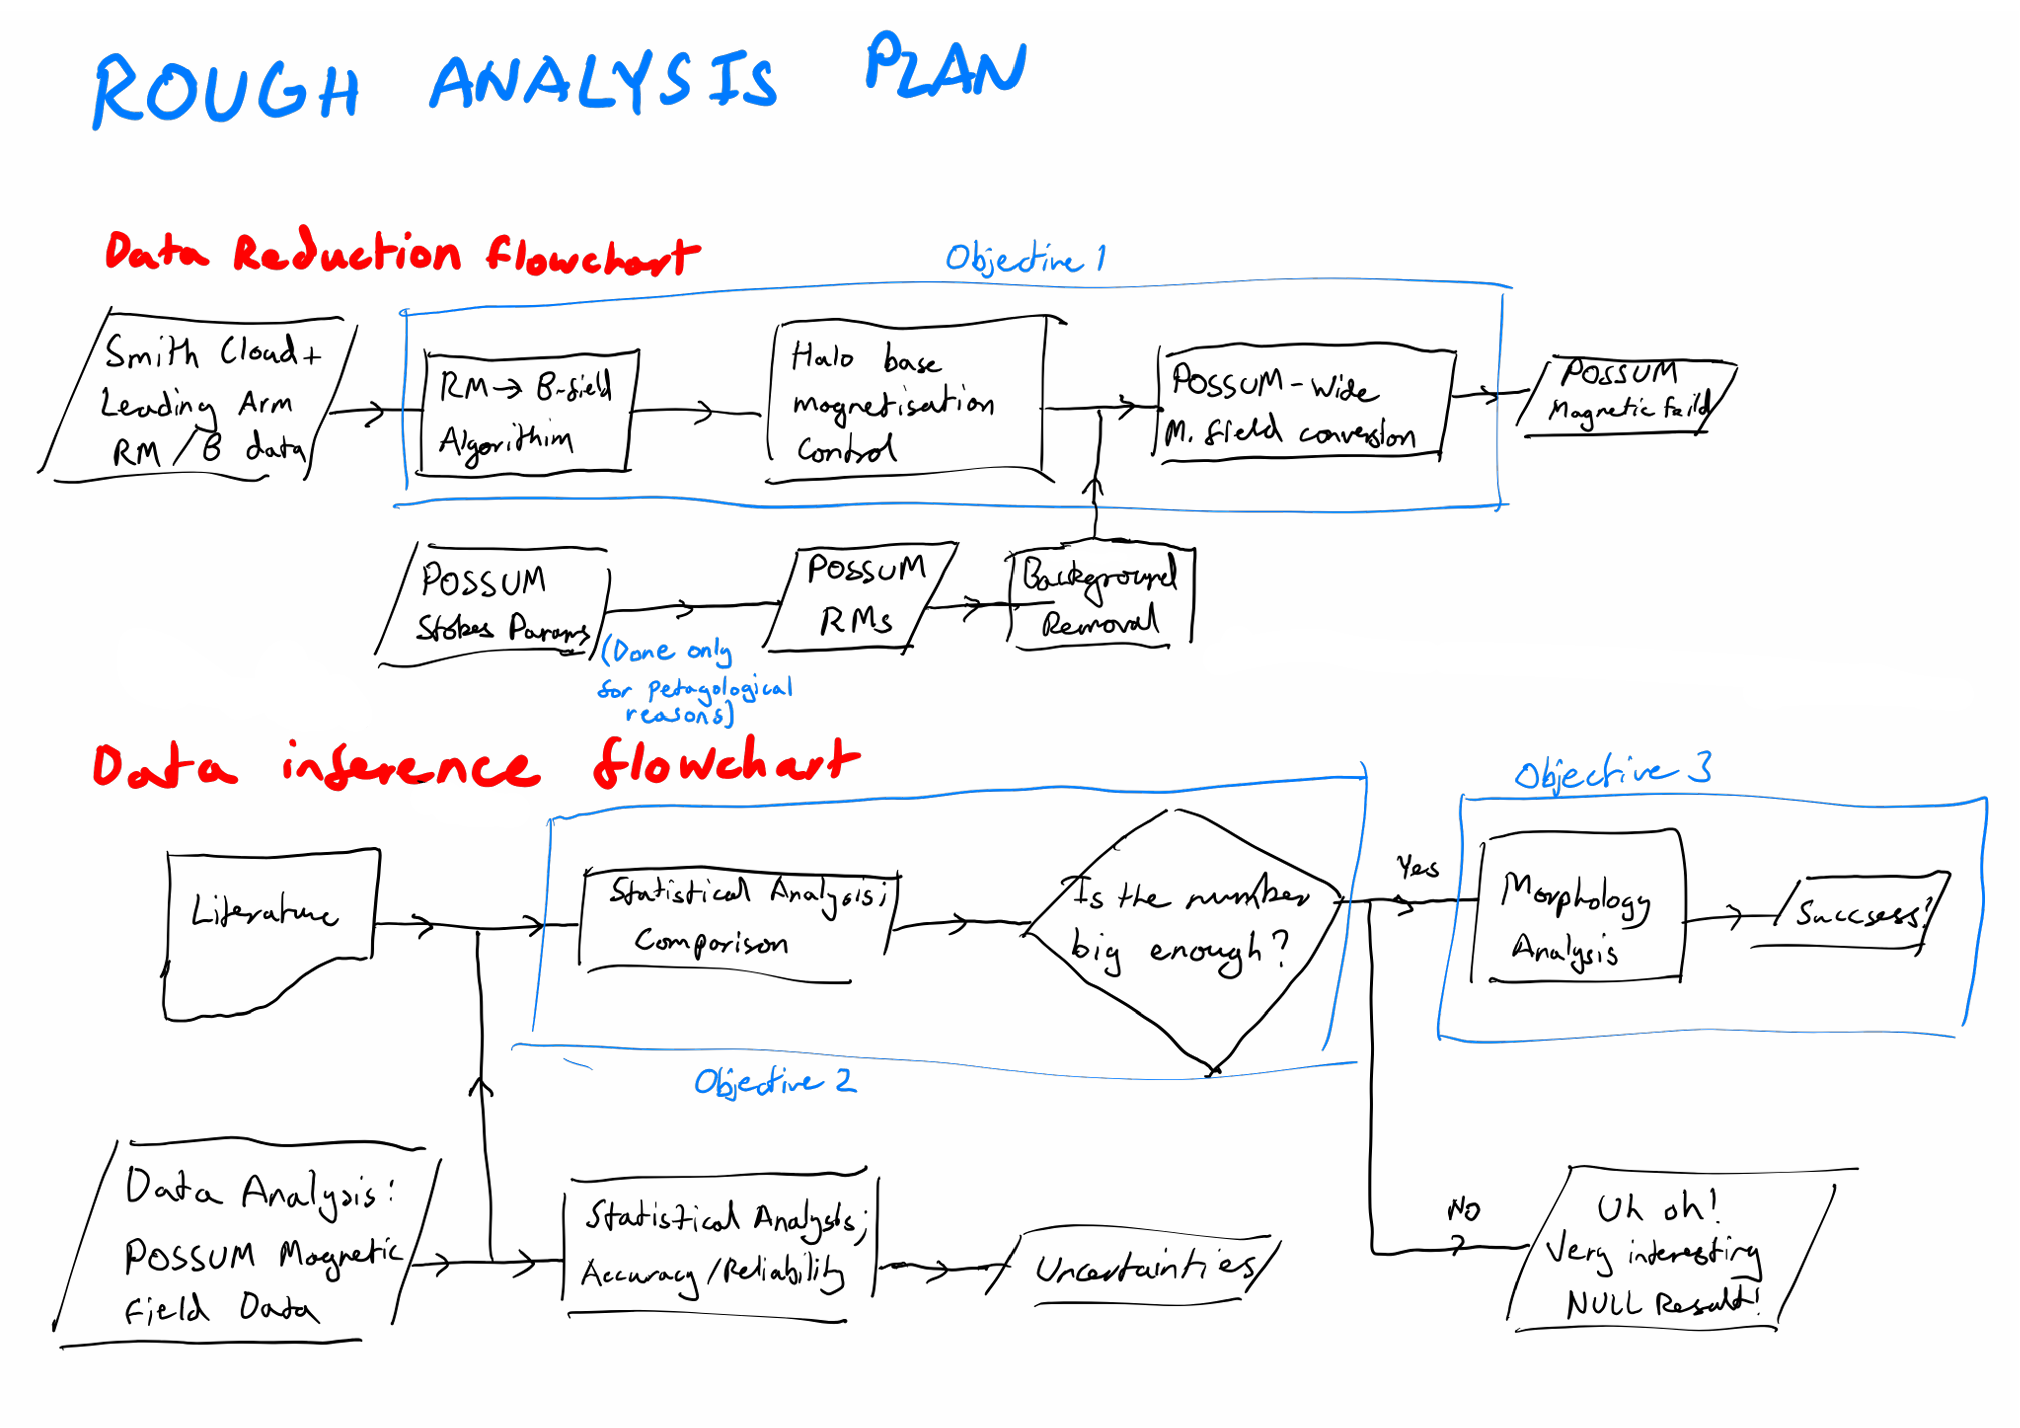
\includegraphics[width=\columnwidth]{figs/flowchart.png}
  \caption{A rough flowchart of the data analysis method. A neater version of this flowchart will appear in future iterations of the report as a visual representation of the methodology.}
\end{figure*}

Figure~\ref{fig:flowchart} represents the rough outline of the pipeline of data analysis as per the three objectives listed in \ref{sec:objectives}.

The first point of data reduction is to convert the raw POSSUM data, i.e. stokes parameters in the field, to rotation measures. A component of research, revision, and programming will be dedicated to doing this. POSSUM as a survey has already condensed the stokes parameters into rotation measures. The purpose of doing it again is purely for pedagogical reasons - so that a better understanding about the nature of RMs is achieved. Purposefully, this part of the data reduction will only appear in perhaps a few sentences in the mid-term and final report, discussing how the POSSUM data was obtained.

Smith Cloud and Leading Arm HVC data will be obtained from a secondary source outside of POSSUM. The purpose of this data is to act as a testing set. Since past research has already determined the magnetic field strengths in HVCs in those regions, along with the base halo magnetisation. It is important that this data be used to confirm that the algorithm developed is working correctly.

After the program is developed to convert rotation measures into magnetic fields, data from the non-active components of the halo itself are then fed through the same algorithm. This will act as a control variable, providing a measure of base magnetisation for the Galactic Halo as well as pointing to a default ionisation state of the halo, which can support HVCs.

The halo control test will also help in the removal of background and foreground sources of Faraday rotation. The light used to measure polarisation comes from extragalactic synchrotron radiation, which is initially unpolarised. However, this radiation will have to travel a far distance before reaching us, at which point it can polarise from any sort of ionised gas in the Universe. HVCs will also be ionised in some manner, and it might be necessary to rely on spectroscopic observations of these HVCs to determine how much they will interfere with incoming light.

All these sources of interference can make it extremely difficult to determine the actual rotation measures in question. A background control run and analysis of the HVC can prevent this issue. RM interference is an active part of the process in radio astronomy, with aforementioned research that aims to tackle this problem. With a larger data set, however, there is more reliability simply because of the scope of data. In previous examples, as mentioned, HVCs in the leading arm can be obscured, which is a way HVCs in the halo can also experience faulty RMs. With more data comes more confidence and a better ability at eliminating outliers.

There are several methods by which one can convert rotation measures to magnetic fields, typically consisting of measuring kurtosis and skew. Other techniques for background removal include convolutional blurring, binned averages, signal whitening/bandpassing. Tools which will be investigated in literature while completing the implementation of objective 1.

Once all these processes are done, the algorithm should be fully capable of a simple pass-over across all HVCs in the entire southern sky. This step is the easiest, as it only involves repeatedly running an already completed script on several objects. After the program is developed, applied across all detected HVCs in the field, and the data is catalogued, the next step is to infer information from this data.

Most of the statistical analysis tools will be very basic, as objective 2 simply requires a rough estimate of the magnetic field strengths. Uncertainties will naturally arise from the program's mathematical evaluations. The K-S test will be used to compare magnetic field distributions to theoretical cases and example cases like the smith cloud. Simple averages, box plots, and other single-set analysis tools will be used to establish a characterisation of the sample. It Is expected, however, that HVCs that are at a higher Galactic latitude will be more resolute as it is less contaminated by dust radio emission from the disk. This should be accounted for in the analysis of uncertainties.

Once these tests have been performed, it will be possible to assess if our results align with the initial alternative hypothesis. From there, either a tertiary objective is completed (if there is time), or further research is recommended in the conclusion of the report.

\section{Timeline of honours project}
\label{sec:timeline}

\begin{table*}[ht]
  \centering
  \input table/timeline.tex
  \caption{A planned timeline of events.}
  \label{tab:timeline}
\end{table*}

Table~\ref{tab:timeline} displays a rough timeline of both honours program milestones and self-assigned objectives.

As a general summary, the first half of the first semester will be focused on initialising the project and starting the process of research and planning. The second half will focus on primarily completing objective 1, in which 14 weeks sounds like a realistic timeframe. The midterm report will be worked on as the tasks of objective 1 start winding down, with all the new research discovered over those months being compiled into the incomplete skeleton of the report.

Objective 2 will require less time, and hence only will take the former half of the second semester. The latter half of the semester is dedicated to drafting and finalising the report and its results. As with any project, after the second semester exams, there will be a bit of time to clean up the project's code for future use, debriefing on the year, and if the research is of enough value, potentially publishing the report.

I do not actually know, according to the honours guidelines, if I am allowed to submit theses for formal publishing after the marking and reviewing of the report internally. At the very least, whether it happens or not, the potential for it to be published will act as a large personal motivator.

There will inevitably be disruptions to the timeline of planned events, in order to account for these several contingency measures are employed:
\begin{enumerate}
\item Starting work on tasks 1-2 weeks before their allocated time
\item Spending a portion of the 20 hrs/week on non-focused tasks (i.e. reading for 3 hrs while working on objective 1)
\item Slightly overestimating the time it takes to complete each aspect of the project, to allow room for slow progress
\item Using a flowchart model of progression, so if one aspect of the project cannot be completed, only future contingencies are hindered
\item Regular and premature testing of programs
\end{enumerate}

%%% Local Variables: 
%%% mode: latex
%%% TeX-master: "paper"
%%% End: 

\chapter{Results}
\label{cha:result}




%\section{Direct Cost}\
%\label{sec:direct_cost}

\lipsum[1] 
%Figure~\ref{fig:cost}
%includes two subfigures (Figure~\ref{fig:zerocost}, and 
%Figure~\ref{fig:zerobus});

%\begin{figure*}
%  \label{fig:cost}
%  \subfigure[Fraction of cycles spent on zeroing\label{fig:zerocost}]%{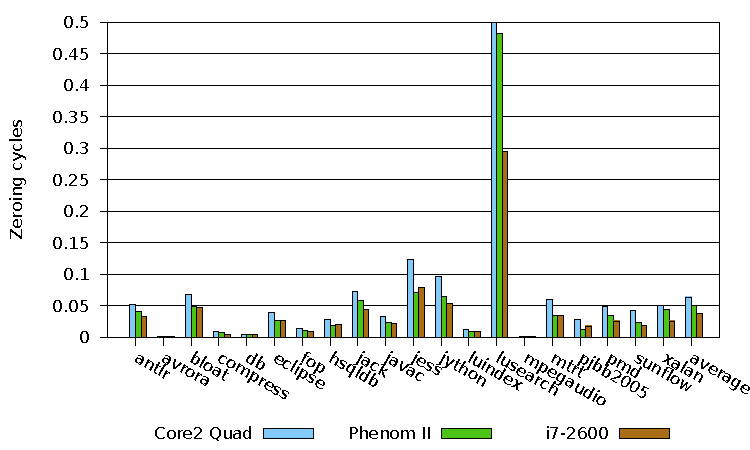
\includegraphics[width=\columnwidth]{figs/zerocost_intel.pdf}}
%  \subfigure[BytesZeroed / BytesBurstTransactionsTransferred\label{fig:zerobus}]{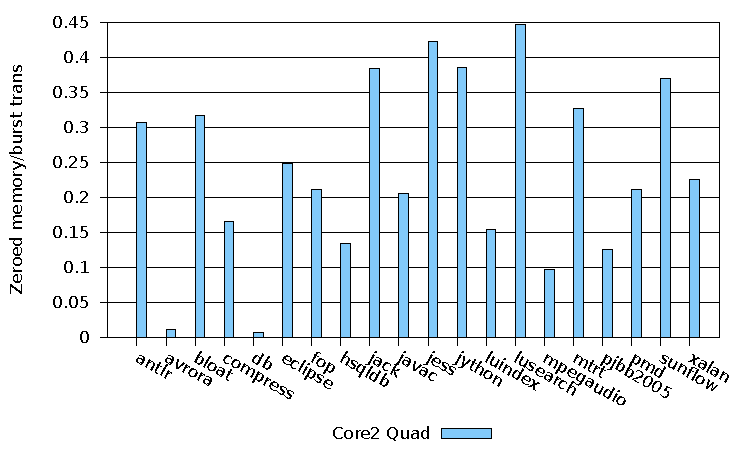
\includegraphics[width=1.0\columnwidth]{figs/zerobus_core.pdf}}
%  \caption{The cost of zero initialization}
%\end{figure*}


%\begin{figure}
%  \centering
%  \subfigure[\label{fig:c:hello}]{
%  \begin{minipage}[b]{\columnwidth}
%    \lstinputlisting[linewidth=\columnwidth,breaklines=true]{code/hello.c}\vspace*{-2ex}
%  \end{minipage}}
%  \subfigure[\label{fig:java:hello}]{
%  \begin{minipage}[b]{\columnwidth}
%    \lstinputlisting[linewidth=\columnwidth,breaklines=true]{code/hello.java}\vspace*{-2ex}
%  \end{minipage}}
%  \caption{Hello world in Java and C.}
%  \label{fig:helloworld}
%\end{figure}

%\section{Summary}

\chapter{Discussion}
\label{cha:discussion}

E

\section{Foreground Removal}
\label{sec:fr_disc}

\begin{itemize}
    \item Edge Detection and Rippling
    \item Comparison of Methods
    \item Sample Size Limitations
\end{itemize}

\subsection{Edge Detection and Rippling}
\label{ssec:A1}

E

\subsection{Comparison of Methods}
\label{ssec:A2}

E

\subsection{Sample Size Limitations}
\label{ssec:A3}

E

\section{Magnetic Field Derivation}
\label{sec:mag_disc}

\begin{itemize}
    \item Data Collection
    \begin{itemize}
        \item HI and H-alpha Data (Not needed!)
    \end{itemize}
    \item Neccesity of Assumptions
    \item Validity of Derivation Methods and VGSR
    \item Uncertainty Analysis
\end{itemize}

\subsection{Data Collection}
\label{ssec:B1}

E

\subsection{Neccesity of Assumptions}
\label{ssec:B2}

E

\subsection{Validity of Derivation Methods}
\label{ssec:B3}

E

\subsection{Uncertainty Analysis}
\label{ssec:B4}

E

\chapter{Conclusions}
\label{cha:conclusion}

E

Also comment on projects in current development. Including \cite{ID70, ID72, ID67}.



%%%%%%%%%%%%%%%%%%%%%%%%%%%%%%%%%%%%%%%%%%%%%%%%%%%%%%%%%%%%%%%%%%%%%%
% Here begins the end matter

\setcounter{chapter}{7}
\setcounter{section}{0}

\renewcommand*{\thechapter}{}

\appendix

\chapter{Appendix}
\label{cha:appendix}

\renewcommand*{\thesection}{\Alph{section}}

\section{Developed code and data}
\label{sec:appendixA}

All developed code and data is found in a publically-available GitHub repository as shown here: \url{https://github.com/Olivex727/hvc-magnetic-honours-programs}.

\section{All HVCs and HVC Calulations}
\label{sec:appendixB}

The filtered Moss catalogue is as below.


\section{Planck Mission Cosmic Microwave Background}
\label{sec:appendixC}

The source for the Planck mission's CMB temperature map is available on this website: \url{https://www.esa.int/ESA_Multimedia/Images/2013/03/Planck_CMB/}.

\section{PyNUFFT Python Module}
\label{sec:appendixD}

The pyNUFFT Python Module, which was used in the investigation for foreground removal, has its main documentation page here: \url{https://pynufft.readthedocs.io/en/latest/index.html}

\section{Statistical ANOVA Tests}
\label{sec:appendixE}

The R language was used to calculate all tests mentioned in \ref{ssec:results_stats}, the file is available here: \url{https://github.com/Olivex727/hvc-magnetic-honours-programs/blob/main/KS_confirmation/wgt_anova.R}.

The specific R code output when running this file is as follows:

\begin{verbatim}
> summary(base_V2_aov)
Df Sum Sq Mean Sq F value Pr(>F)  
data_new$variable.x  2   44.7  22.349   3.375 0.0388 *
Residuals           87  576.1   6.622                 
---
Signif. codes:  0 '***' 0.001 '**' 0.01 '*' 0.05 '.' 0.1 ' ' 1
> tukey.test
Tukey multiple comparisons of means
95% family-wise confidence level

Fit: aov(formula = data_new$Estimate ~ data_new$variable.x,
weights = data_new$prescision)

$`data_new$variable.x`
   diff       lwr         upr     p adj
Var_Sub-KS_EDF   -1.199 -2.783335  0.38533482 0.1741072
Wgt_Mean-KS_EDF  -1.675 -3.259335 -0.09066518 0.0357301
Wgt_Mean-Var_Sub -0.476 -2.060335  1.10833482 0.7544765

> 
\end{verbatim}

A copy of this text output is available in the file: \url{https://github.com/Olivex727/hvc-magnetic-honours-programs/blob/main/KS_confirmation/chisq.txt}.

\backmatter

\bibliographystyle{anuthesis}
\bibliography{thesis, batch1, batch1additional}

\printindex

\end{document}
